28. \begin{figure}[ht!]
\center{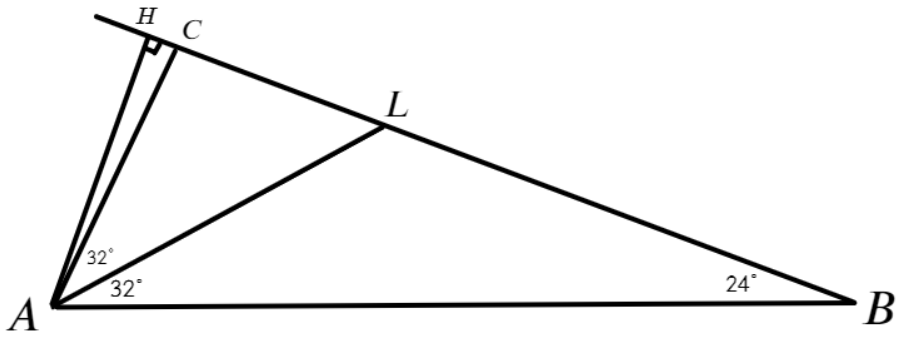
\includegraphics[scale=0.35]{g28.png}}
\end{figure}\\
$\angle C=180^\circ-\angle A-\angle B=180^\circ-64^\circ-24^\circ=92^\circ.$ Так как $\angle C>90^\circ,$ высота из точки $A$ падает на продолжение стороны $BC.$   Пусть $AH$ высота, а $AL$ --- биссектриса. Тогда $\angle CAH=90^\circ-\angle HCA=90^\circ-(180^\circ-\angle C)=90^\circ-88^\circ=2^\circ,$ а $\angle CAL=64^\circ:2=32^\circ.$ Таким образом, $\angle LAH=\angle CAL+ \angle CAH=32^\circ+2^\circ=34^\circ.$\newpage\noindent
